% Source: fixed 2015 Hunan science paper, printed page 956.
% Schematic vector redraw; preserves labeled incidence/hidden-edge topology only.
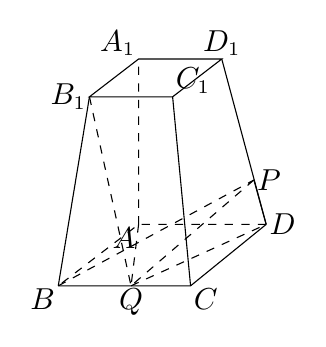
\begin{tikzpicture}[scale=1.2, every node/.style={font=\fontsize{10.5pt}{12.6pt}\selectfont, inner sep=1pt}]
  \coordinate (A) at (0,0);
  \coordinate (B) at (-.85,-.65);
  \coordinate (C) at (.55,-.65);
  \coordinate (D) at (1.35,0);
  \coordinate (Aone) at (0,1.75);
  \coordinate (Bone) at (-.52,1.35);
  \coordinate (Cone) at (.36,1.35);
  \coordinate (Done) at (.88,1.75);
  \coordinate (P) at (1.22,.47);
  \coordinate (Q) at (-.08,-.65);
  % Lower and upper square bases and visible frustum edges.
  \draw (B)--(C)--(D);
  \draw[dashed] (D)--(A)--(B);
  \draw (Bone)--(Cone)--(Done)--(Aone)--cycle;
  \draw (B)--(Bone) (C)--(Cone) (D)--(Done);
  % Hidden edges and the construction segment shown in the source.
  \draw[dashed] (A)--(Aone) (Bone)--(Q) (A)--(Q) (B)--(P) (P)--(Q) (Q)--(D);
  \draw (D)--(P);
  \foreach \pt/\pos/\lab in {A/below left/A,B/below left/B,C/below right/C,D/right/D,
      Aone/above left/A_1,Bone/left/B_1,Cone/above right/C_1,Done/above/D_1,P/right/P,Q/below/Q}
    \node[\pos] at (\pt) {$\lab$};
\end{tikzpicture}
